
\newglossaryentry{X}
{
  type=differential-privacy,
  name={$\ensuremath{X} $},
  description={Set of locations for a user. ($R^2$)},
}
\newglossaryentry{Z}
{
  type=differential-privacy,
  name={$\ensuremath{Z} $},
  description={For every $x \in X$ a perturbed location $z \in Z$ is reported.},
}
\newglossaryentry{K}
{
  type=differential-privacy,
  name={$K(x)(Z)$},
  description={Randomization method for $x \in X$ and output $z \in Z$.},
}
\newglossaryentry{Epsilon}
{
  type=differential-privacy,
  name={$\ensuremath{\epsilon} $},
  description={The privacy budget $\epsilon$ determines the amount of noise that is added.
    },
}
\newglossaryentry{Pr}{
  type=differential-privacy,
  name={$Pr(K(x_i) \in (Z))$},
  description={Probability of reporting $x \in X$ for $z \in Z$}
}


\section{Differential privacy} \label{section:dp}
In practice, data is often sent to a central storage point.
This requires trust, and because all data is collected in one place, the risk of private data leakage becomes very high.
By applying differential privacy, noise can be added to the data to protect it.
This is principle is illustrated in figure \ref{fig:central-dp} with the following actors:
\begin{enumerate}
  \item Trusted curator: The system that receives data from users. It is assumed in this setting that the system is trustworthy and that the data is securely stored.
  \item Adversary: An adversary is someone who uses the data. This could be, for example, a data scientist who wants accurate results, or an attacker who wants to obtain as much data as possible.
  \item The users are clients (for example, websites or mobile apps) who entrust their data to a central server.
\end{enumerate}
With the introduction of differential privacy, the privacy of a user would be ensured (to a certain extent).
This will be further explained in the next section.

Although differential privacy solves many problems (as mentioned earlier in the introduction), it remains difficult to calibrate the mechanism.
There is an important trade-off between utility and privacy for the adversary, where a data scientist wants accurate data while the noise must be sufficient to prevent an attacker from obtaining too much information.
For this reason, the following chapters will be devoted to outlining the mathematical background of differential privacy.
We will examine which factors influence this calibration and whether other methods contribute to it.
Afterward, we will also further explain other types of differential privacy (local and geo-indistinguishable) in the same way.
\begin{figure}[h!]
  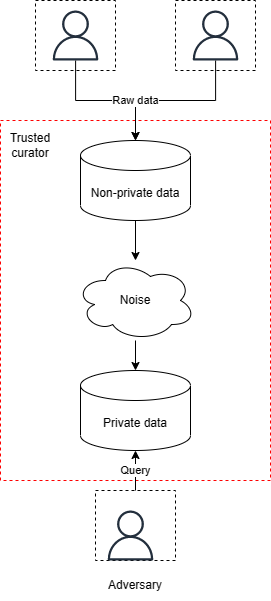
\includegraphics[width=0.2\textwidth]{TheorethicalFramework/Differential privacy/central-dp.png}
  \caption{General approach for setting up (central) differential privacy.}
  \label{fig:central-dp}
\end{figure}
%\glsaddall
%\leading{10pt}
%\printglossary[type=differential-privacy, nonumberlist]
%\begin{figure}[h]
%  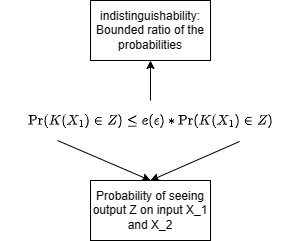
\includegraphics{TheorethicalFramework/Differential privacy/master-thesis-Differential privacy illustration.png}
%  \caption{Randomization function $K$ gives $\epsilon$-differential privacy for all elements in $D_1$ and $D_2$ if they differ at most one element. \citep{dwork_differential_2006}}
%  \label{fig:definition-dp}
%\end{figure}

\newpage
\subsection{Definitions}
We examine the different notations and types of differential privacy we consider in this research.

\subsubsection{$\epsilon$-differential privacy}
Dwork et al formulated the notion of privacy as: Participating in a database should not significantly increase the risk of an individual's privacy being compromised \cite{dwork_differential_2006}.
This is mathematically formulated in the same research with the name \gls{dp}.
Using the definition of privacy, it is formulated as the maximal possible change when adding or removing a single record \citep{dwork_differential_2006, friedman_data_2010}.
This is reflected using the formal mathematical formulation as formulated by dwork et al:
\begin{equation}
  {\mathrm{Pr}}[K(D_{1})\in S]\leq\exp(\epsilon)\times{\mathrm{Pr}}[K(D_{2})\in S]
  \label{pure-dp}
\end{equation}
So, given a randomization function $K$, it gives $\epsilon$-differential privacy if dataset $D_1$ and $D_2$ are differing at most one element \citep{dwork_differential_2006}.
The $\epsilon$ determines the amount of noise (privacy budget) \citep{friedman_data_2010}.
The lower the value of $\epsilon$ means, the higher the privacy guarantee.
In this regard, it is important for a method that ensures differential privacy to take this into account.
For this reason, a common way to determine the $\epsilon$ is to calculate the sensitivity.
This value is calculated based on the impact of a function or query on the data.
For example, if there is a method called $sum$ for the summation of data points, the sensitivity of the method is 1.
This is because removing one data point would greatly affect the outcome and $\epsilon$-differential privacy could no longer be guaranteed.
It is also mathematically defined by dwork et al:
\begin{equation}
  \Delta f=\operatorname*{max}_{D_{1},D_{2}}\|f(D_{1})-f(D_{2})\|_{1}
  \label{sensitivity-dp}
\end{equation}
\subsubsection{$(\epsilon, \delta)$-differential privacy}
The formal notion of differential privacy has only $\epsilon$ input.
This formulation is really strict, but most methods relax this a little which is defined as $(\epsilon, \delta)$.
\begin{equation}
  {\mathrm{Pr}}[K(D_{1})\in S]\leq\exp(\epsilon)\times{\mathrm{Pr}}[K(D_{2})\in S] + \delta
  \label{approxiate-dp}
\end{equation}
This means the sensitivity (now denoted as delta $\delta$) is used to loosen up the definition.
The purpose of $\epsilon$ now is to calibrate the desired amount of privacy.
To some extent, the delta represents the probability of the algorithm leaking information \citep{aitsam_differential_2021}.
With $\epsilon$-differential privacy, there would be no difference in the case of information leakage (delta = 0).
However, with $(\epsilon, \delta)$-differential privacy, the information can leak up to the probability of delta.

\subsubsection{$\epsilon$-local differential privacy}
As the name suggests, \gls{ldp} is executed on the client-side instead of on the server, as was the case in figure \ref{fig:central-dp}.
This is illustrated in figure \ref{fig:local-dp}.
Local differential privacy was introduced to remove the "trusted" curator, preventing sensitive data leakage even if an attacker gains access to the dataset \citep{del_rey_comprehensive_2020-1}.
The definition for \gls{ldp} is the as for equation \ref{approxiate-dp} with $\delta = 0$ being equal to equation \ref{pure-dp}.
\todo[inline]{Describe issues with local differential privacy}
\begin{figure}[h]
  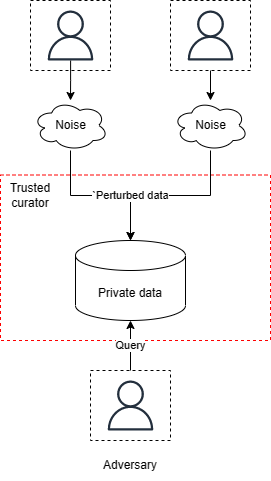
\includegraphics[width=0.3\textwidth]{TheorethicalFramework/Differential privacy/master-thesis-Pagina-8.png}
  \caption{Local differential privacy, which moves the noise-adding step to the client-side.}
  \label{fig:local-dp}
\end{figure}
\subsubsection{$\epsilon$-geo-indistinguishability}
The last and for this study's most important type of differential privacy is \gls{gi}.
This is a type of differential privacy that is specifically designed for location data.

\subsection{Mechanisms}
In this section, we will explain the various mechanisms that are used to achieve differential privacy.
The different mechanisms are not limited to the type of \gls{dp} and some can be applied to multiple types.
%The mechanisms are divided into three categories: \gls{dp}, \gls{ldp} and \gls{gi}.
\subsubsection{Randomized response mechanism}
The random response method is a relatively simple method and was first applied in 1965 by Warner et al.
It was originally used to mask the answers of individuals by randomly switching the answers with predictable randomness \citep{warner_randomized_1965-1}.
Therefore, the method is mainly used for categorical data.
This method satisfies its own set of requirements for LDP \citep{del_rey_comprehensive_2020-1}, which differs from the formal definition that was mentioned earlier

Since then, it is still one of the better-known methods, and larger organizations such as Google use it \citep{erlingsson_rappor_2014-2}.
They have named their extension RAPPOR and expanded it with bloom filters to be able to collect numerical data as well.
It has been possible to ensure $\epsilon$-differential privacy in this way, and it is also possible to preserve \gls{ldp} \citep{del_rey_comprehensive_2020-1}.
\subsubsection{Laplace mechanism} \label{laplace}
The method that was originally proposed in the differential privacy paper by Dwork et al. is the Laplace algorithm \citep{dwork_differential_2006}.
Therefore, the method works by configuring the $\epsilon$ and $\delta$. A shorthand definition is provided by Rey et al \citep{del_rey_comprehensive_2020-1}:
\begin{equation}
  M\left(f\left(x\right),\varepsilon\right)=f\left(x\right)+\left(Z_{1},\ldots,Z_{d}\right)
\end{equation}
The mechanism is based on the Laplace distribution with scale $\lambda f/\epsilon$, where $\lambda f$ is the same as in equation \ref{sensitivity-dp}.
Therefore, the Laplace mechanism is tightly linked to the definition of pure-dp and so it is $\epsilon$-differential privacy \citep{dwork_differential_2006}.
It is also suitable for preserving \gls{ldp} \citep{del_rey_comprehensive_2020-1}.
One disadvantage is that sensitivity is always required, and this parameter can sometimes be difficult to configure.
Especially when there is no clear function and the entire dataset is perturbed.
This can make it challenging to find the right balance between ensuring privacy and utility.

To this end, the sensitivity can be calculated in two forms: global and local.
Global sensitivity is calculated over two different datasets and is part of the original definition of \gls{dp} \citep{dwork_differential_2006}.
It is called global because it is independent of the queried dataset.
Usually, this is not the desired situation, since local sensitivity always has more context of the dataset in question \citep{nissim_smooth_2007}.
As a result, the trade-off for noise is much more precise, and the balance between utility and privacy is much better.
This local sensitivity definition \citep{nissim_smooth_2007}.
\begin{equation}
  LS(f,x)=\operatorname*{max}_{x^{\prime}\cdot d(x,x^{\prime})\leq1}|f(x)-f(x^{\prime})|
  \label{local-sensitivity}
\end{equation}
A methodology to calculate the local sensitivity is by using the smooth sensitivity method, which was proposed by the same authors \citep{nissim_smooth_2007}.
This method aims at smoothing out the local sensitivity by focusing on reducing the noise.
The goal is to smooth out the amount of noise, to reduce the risk of something being revealed in the data.
Due to this, a disadvantage of this method is that it can be computationally expensive.
Also, the introduction of this method makes Laplace preserve $(\epsilon, \delta)$-\gls{dp} instead of pure $\epsilon$-\gls{dp}.

\subsubsection{Gaussian mechanism} \label{gaussian}
Another mechanism that works comparably is the Gaussian mechanism.
This mechanism makes use of the Gaussian distribution to add noise to the data.
% This means, that if the sensitivity is low, the noise is as well.
% The metric is combined with the privacy budget $\epsilon$ to control the noise that is being added by a mechanism like Laplace \citep{friedman_data_2010}.


%The above attacks mainly target the clustering method after they have been trained. 
%$Various attacks are more focused on data, like 
%\subsection{Evaluation methods} \label{theory:evaluation-dp}
\mycomment{
  It is possible to evaluate and measure the impact of the noise between two distributions by calculating the error between the non-private and private data \citep{del_rey_comprehensive_2020-1}.
  Two metrics that are proposed by the same study are Mean Squared Error (MSE) and Mean Average Error (MAE).
  These metrics can be used to calculate the error between $X$ and the perturbed dataset $Z$. \newline

  Just as it is possible to measure the utility, this can also be done with privacy.
  When performing a privacy algorithm, it can be proven whether a method meets the privacy requirements.
  These are metrics such as $\epsilon$-differential-privacy (\ref{fig:definition-dp}) and $\epsilon$-geo-indistinguishability (see next chapter \ref{algo:2d-geo-indistinguishability}).
  Although these methods give an idea of privacy, it can only be "yes" or "no".
  Furthermore, it can give a distorted image, since a chance of 70\% also gives a "yes" according to the definition of geo-indistinguishability \citep{oya_is_2017}.
  In other words, to gain more insight into the amount of privacy (such as with MSE or MAE), other metrics are needed.

  For this reason, Oya et al. introduced a metric for geo-indistinguishability that makes it possible to give percentages in their study \citep{oya_is_2017}:
  As an example, an adversary is given that guesses between two locations: $x \in X$ and  $x' \in X$.
  \begin{equation}
    p_e (x, x', z) \leq p^*_e = \frac{1}{1 + e^{e * d(x, x')}}
    \label{eq:geo-as-an-error}
  \end{equation}
  Where privacy level $p^*_e$ is the lower bound of the probability of an adversary guessing correctly.
  The method is called $\epsilon$-geo-indistinguishability as error.
  Based on this metric, it can be calculated that an adversary has an average of 90\% chance to guess a location correctly.
  In that case, the algorithm would be $\epsilon$-geo-indistinguishability, but in practice not.
}